%// !TEX program = luatex
% luatex %.tex|"yourPDFreaderProgramExecutable" %.pdf
\documentclass[11pt]{beamer}
\usepackage{csquotes}
\usepackage{polyglossia}
\setdefaultlanguage{german}
%für luatex
\usepackage{luatextra}
\usepackage{luacode}
\usepackage{fontspec}

\usepackage{setspace}
\usepackage{supertabular}
\usepackage{graphicx}

\usepackage{float}
\usepackage{amsmath}
\usepackage{amssymb}
\usepackage{thmtools}
\usepackage{enumitem}
\usepackage{color}
\usepackage[font=footnotesize]{caption}
\usepackage{url}

\usefonttheme[onlymath]{serif}

\usepackage[backend = biber]{biblatex}
\bibliography{\jobname}
\usepackage{filecontents}
\begin{filecontents}{\jobname.bib}
@misc{*cite*,
title = {{*Titel*}},
howpublished = {\url{*url*}},
note = {Zugegriffen: *Datum*},
}
\end{filecontents}


\title{Matrixgruppen}

\author{Jan Hurt\\
		Betreuer: Cap Andreas}

\date{\small{Datum: 27.11.2015}}
\titlegraphic{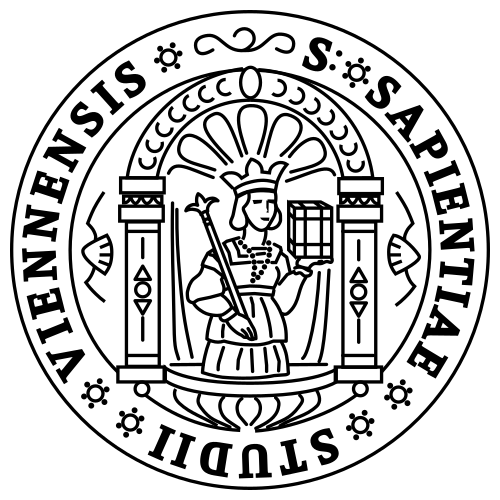
\includegraphics[width=0.35\textwidth]
{Uni_wien_siegel.png}}



\begin{document}
\begin{frame}
\titlepage
\end{frame}

\begin{frame}
	\frametitle{Gruppen von Matrizen}
	Folgende Teilmengen der Matrizen $M_n(\mathbb{K})$
	($\mathbb{K}$ ist $\mathbb{R}$ oder $\mathbb{C}$) bilden mit der Operation
	$(A,B) \mapsto AB$ eine Gruppe. \pause
	\begin{enumerate}[label = $(\roman*)$]
	\item $GL_n(\mathbb{K}) := \{A \in M_n(\mathbb{K}): \det(A) \neq 0 \}$ \\[0.5em] \pause 

	\item $SL_n(\mathbb{K}) := \{A \in M_n(\mathbb{K}): \det(A) = 1 \}$ \\[0.5em]

	\item $O(n) := \{A \in M_n(\mathbb{R}): AA^T = \mathbb{I} \}$ \\[0.5em]

	\item $U(n) := \{A \in M_n(\mathbb{C}): AA^T = \mathbb{I} \}$ \\[0.5em]

	\item $SO(n) := \{A \in M_n(\mathbb{R}): AA^T = \mathbb{I} \wedge \det(A) = 1  \}$ \\[0.5em]

	\item $SU(n) := \{A \in M_n(\mathbb{C}): AA^* = \mathbb{I} \wedge \det(A) = 1 \}$ \\[0.5em]
	\end{enumerate}
\end{frame}

\begin{frame}
	\frametitle{Motivation:}
	Die $GL_n(\mathbb{K})$ sind offen in $M_n(\mathbb K)$. \\ [1em] \pause 
	Die folgenden Operationen: 
	\begin{enumerate}[label = $(\roman*)$]
		\item $GL_n(\mathbb{K}) \times GL_n(\mathbb{K}) \to GL(\mathbb K)$ definiert durch $(A,B) \mapsto A\cdot B$ \pause
		
		\item $^{-1}:GL_n(\mathbb{K}) \rightarrow GL_n(\mathbb{K})$ defniniert durch: $A\mapsto A^{-1}$
	\end{enumerate}
	glatt. \pause 
	Denn in den Einträgen der neuen Matrix stehen nur Polynome der
	ursprünglichen. \\[1em] \pause 
	Die $SU(2)$ ist isomorph zu $S^3 :=\{ x \in \mathbb{R}^4: \|x\|_2 = 1\}$. \pause 
	Denn, ist $A \in SU(2)$ so
	$\exists \alpha, \beta \in \mathbb{C}$ sodass
	$A = \left( \begin{matrix} \alpha & -\bar{\beta} \\ \beta  & \bar{\alpha}\end{matrix} \right)$
	mit der Bedingung $\det(A) = |\alpha|^2 + |\beta|^2 =
	Re(\alpha)^2 + Im(\alpha)^2 + Re(\beta)^2 + Im(\beta)^2$ = 1. \\[1em]
\end{frame}

\begin{frame}
	\frametitle{Matrixgruppen}
	\textbf{Definition:}
	Eine Matrixgruppe ist eine abgeschlossene
	Untergruppe von $GL_n(\mathbb{K})$. \\[1em] \pause

	\textbf{Beispiele:}
	Da $f:A \mapsto AA^*$ stetig ist, ist $O(n) = f^{-1}(\mathbb{I})$ abgeschlossen
	und daher eine Matrixgruppe. Genauso $SO(n),U(n), SU(n)$. \\[1em]
\end{frame}

\begin{frame}
	\frametitle{Tangentialräume}
	\textbf{Definition:}
	Ist $G$ eine Matrixgruppe, so ist
	\begin{align*}
		\mathfrak{g} := \{ \alpha'(0): & \;\; \alpha:(-\varepsilon, \varepsilon) \rightarrow M_n(\mathbb{K}) \text{ glatt},\\ 							
										&\text{ mit } \alpha(0) = \mathbb{I}, \text{ und } \alpha((-\varepsilon, \varepsilon)) \subseteq G\} (*)
	\end{align*}
  der Tangentialraum von $G$ bei $\mathbb{I}$.
\end{frame}


\begin{frame}
	\frametitle{Einparameteruntergruppen}
	\textbf{Definition:}
	Eine Einparmeterunteruppe ist ein einer Gruppe $G$ ist eine Abbildung:
	$\alpha:\mathbb{K} \rightarrow G$, sodass $\forall s, t \in \mathbb{K}$ gilt
	$\alpha(s+t) = \alpha(s)\cdot \alpha(t)$. \\[1em] \pause
	
	\textbf{Definition:}
	Für $A \in M_n(\mathbb{K})$ ist $\exp: M_n(\mathbb K) \to GL_n(\mathbb K)$:
	\begin{align*}
	\exp(A) = e^A := \sum_{n = 1}^{\infty} \frac{A}{n!}.
	\end{align*} \pause
	\textbf{Bemerkung:}
	Es gilt $\forall s,t\in \mathbb K: \exp((s+t)A) = \exp(sA) \exp(tA)$, Beweis wie im reellen/komplexen Fall über Binomischen Lehrsatz ($(s+t)A = (t+s)A$) $\Rightarrow$ $t\mapsto e^{tA}$ ist eine Einparameteruntergruppe.
\end{frame}

\begin{frame}
	\textbf{Lemma:}
	Es gilt, dass die glatten Einparameterungergruppen in $GL_n(\mathbb{K})$ genau die Abbildungen $t\mapsto e^{tX}$ für $X\in M_n(\mathbb{K})$ sind. \\[1em] \pause

	\textbf{Beweis:}
	Sei $\alpha$ eine Einparameteruntergruppe, so definiere $X:=\alpha(0)'$, \pause
	dann gilt $\alpha(t)' = \frac{d}{ds}\Big\vert_{s=0}\alpha(t+s) = \frac{d}{ds}\Big\vert_{s=0} \alpha(t)\alpha(s) = \alpha(t)\alpha'(0) = \alpha(t)X$,\pause
	 genauso $(e^{tX})' = e^{tX}X$ \pause
	außerdem gilt $\alpha(0) = \mathbb{I} = e^0$
	$\Rightarrow$ da die die Abbildungen die selbe Differentialgeichung erfüllen, sind sie ident: $e^{tX} = \alpha(t)$ \\[2em] \pause

	\textbf{Satz:}
	Es existieren offene Umgebungen von $0\in V \subseteq M_n(\mathbb{K})$ und $\mathbb{I}\in U\subseteq M_n(\mathbb{K})$, sodass $X\mapsto e^X$ eine glatte Bijektion $V\to U$ ist und deren Inverse ebenfalls glatt ist.\\[1em] \pause
	
	\textbf{Beweis:}
	Folgt aus dem Inverse Funktionen Satz da $(e^X)'\big\vert_{X=0} = \mathbb{I}$.
\end{frame}

\begin{frame}
	\textbf{Satz:}
	Sei $G\subseteq GL_n(\mathbb{K})$ eine Matrixgruppe, $\mathfrak{g}\subseteq M_n(\mathbb{K})$ wie oben, dann gilt \pause
	\begin{enumerate}[label = $(\roman*)$]
		\item $\mathfrak{g}$ ist ein Teilraum und $\mathfrak{g} = \{ X\in M_n(\mathbb{K}):\; \forall t:e^{tX}\in G \}$ \pause
		
		\item $\exists$ offene Umgebungen $V$ von 0 in $M_n(\mathbb{K})$, $U$ von $\mathbb{I}$ in $GL_n(\mathbb{K})$, sodass $\exp$ zusätzlich $V\cap \mathfrak{g}$ bijektiv auf $U\cap G$ abbildet. \pause
	\end{enumerate}
	
	\textbf{Beweis:} $(i)$ Sind $\alpha$, $\beta$ Kurven die $(*)$ erfüllen und
	$\gamma(t):= \alpha(t)\beta(t)$. Dann gilt: \pause
	\begin{equation*}
	\gamma'(0) = \alpha'(0)\beta(0) + \alpha(0)\beta'(0) = \alpha'(0)+\beta'(0).
	\end{equation*} \pause
	Ist $r\in \mathbb{K}$ und $\gamma(t) := \alpha(rt)$ dann ist
	$\gamma'(t) = r\alpha'(rt)$, also $\gamma'(0) = r\alpha'(0)\in \mathfrak{g}$. \\[0.5em]
\end{frame}

\begin{frame}
		\textbf{Definition:}
		Eine Funktion $f: G\to M_n(\mathbb{K})$ ist lokal um einen Punkt $g \in G$ glatt $:\Leftrightarrow$ die Abbildung $X \mapsto f(ge^X)$ ist glatt auf der offenen Teilmenge $V \cap \mathfrak g \subseteq \mathfrak g = M_n(\mathbb{K})$. \\[1em] \pause
		Sind $G, H$ Matrixgruppen, $G,H \subseteq M_n(\mathbb{K})$ so ist der Homomorphismus $\Phi:G \to H$ glatt $:\Leftrightarrow$ die Funktion $\Phi:G \to M_n(\mathbb{K})$ ist glatt.
\end{frame}

\begin{frame}
	Ist $\alpha$ eine Kurve die $(*)$ erfüllt, und ist $\Phi:G \to H$ ein glatter Homomorphismus so ist die Kurve $\Phi\circ\alpha$ glatt in $H$ und $\varphi$ definiert über:  $\varphi(\alpha'(0)) = (\Phi\circ\alpha)'(0)$ ist wohldefiniert. \\[1em] \pause
	\textbf{Proposition:}
	Ist $\Phi, \varphi$ wie oben definiert, so gilt $\Phi(e^X) = e^{\varphi(X)}$.
	Daraus folgt, dass $\Phi$ lokal um $\mathbb{I}$ eindeutig durch $\varphi$ bestimmt. \\[1em] \pause
	\textbf{Beweis:}
	$\Phi(e^{tX})$ ist eine Einparameteruntergruppe mit $(\Phi(e^{tX}))'\big\vert_{t=0} = \varphi((e^{tX})'\big\vert_{t=0}) = \varphi(X(e^{tX})\big\vert_{t=0}) = \varphi(X)$.	
\end{frame}


\begin{frame}
	\textbf{Propostion:}
	Ist $H$ zusammenängend so ist die von $exp(\mathfrak{h})$ erzeugte Untergruppe isomorph zu $H$.\\ [1em] \pause 
	\textbf{Beweis:}
	Die Teilmenge $U\cap H$ vom obigen Satz liegt in $\exp(\mathfrak h)$ und damit in der davon erzeugte Untergruppe $\tilde H\subset H$. \\ \pause
	Analog liegt für $h\in\tilde H$ die Menge $hU\cap H$ in $\tilde H$ (wobei $hU = \{hg:g\in U\}$).
	Nun ist aber nach Definition jede dieser Teilmengen offen in $H$,\pause
	 also ist $\tilde H$ eine offene Teilmenge von $H$. 
	Das Komplement von $\tilde H$ in $H$ ist aber eine Vereinigung von Nebenklassen, die jeweils
	isomorph zu $\tilde H$, also ebenfalls offen. \pause
	Somit ist $\tilde H$ auch abgeschlossen, und weil H
	zusammenhängend ist, folgt $\tilde H=H$. \\[1em] \pause
	
	\textbf{Korrolar:}
	Ist $\Phi:G \rightarrow H$ ein glatter Homomorphismus, $\varphi$ surjektiv
	und $H$ zusammenängend dann ist $\Phi$ surjektiv. \\[1em]
\end{frame}

\begin{frame}
	\textbf{Anwendung:} 
	Man beobachtet, dass $\mathfrak{su(2)} = \left\{ \left( \begin{matrix}
	a  	& -b+ic\\
	b+ic	& -ia
	\end{matrix}\right): a,b,c \in \mathbb{R} \right\} \cong \mathbb{R}^3$ 
	ist \pause
	und 
	$\langle X, Y \rangle:= -spur(XY)$ ein positiv definites Skalarprodukt auf $\mathfrak{su(2)}$\pause 
	definiert.
	Weiters gilt für $A\in SU(2)$, $X\in \mathfrak{su(2)}$, dass $AXA^{-1} \in \mathfrak{su(2)}$,\pause
	 und 
	$Ad_A:\mathfrak{su(2)} \to \mathfrak{su(2)}$ definiert durch $Ad_A(X) := AXA^{-1}$ erhält das Skalarprodukt und ist deshalb orthogonal bzgl. $\langle \,\, , \, \rangle \Rightarrow Ad_A \in SO(3)$ ist. \\ \pause
	
	 
	$\Phi: SU(2) \to SO(3)$, $\Phi(A) := Ad_A$ ist glatt und surjektiv, da die zugehörige Abbildung $\varphi$ bijektiv ist. \pause
	Da $Ker(\Phi) = {\pm \mathbb{I}}$ ist, folgt dass $SO(3)$ isomorph zu $SU(2)/\{\pm\mathbb{I}\}$ ist.
	
\end{frame}

\begin{frame}
	\frametitle{Lie-Homomorphismen}
	\textbf{Definition:}
	Die bilineare Abbildung $[X, Y] := XY - YX$ wird Kommutator oder Lie-Klammer bezeichnet.\\[1em] \pause
	\textbf{Proposition:}
	Ist $\varphi$ wie in der obigen Propositon, und sind $X, Y \in \mathfrak{g}$ so gilt: \pause
	\begin{enumerate}[label = $(\roman*)$]
		\item $A\in G, X \in \mathfrak g \Rightarrow AXA^{-1} \in \mathfrak g$ \pause
		
		\item $X, Y \in \mathfrak g \Rightarrow [X,Y] \in \mathfrak g$ \pause
		
		\item $\forall X \in \mathfrak{g}, g\in G$ gilt $\varphi(gXg^{-1}) = \Phi(g) \varphi(X) \Phi(g)^{-1}$ \pause
		
		\item $\forall X, Y \in \mathfrak{g}$ gilt $\varphi([X,Y]) = [\varphi(X), \varphi(Y)]$ \pause
	\end{enumerate}
	
	\textbf{Beweis:}
	$(i)$ $X\in \mathfrak g \Rightarrow e^{tX}\in G\; \forall t \Rightarrow Ae^{tX}A^{-1} \in G$ ist Einparameteruntergruppe, mit Ableitung $AXA^{-1} \Rightarrow AXA^{-1} \in \mathfrak g$ \\[1em]\pause
	$(ii)$ Aus $(i)$ folgt: $e^{tX}Ye^{-tX} \in \mathfrak g\; \forall t \Rightarrow [X,Y] \in \mathfrak g$
	
\end{frame}

\begin{frame}
	\textbf{Beweis:}
	$(iii)$ Ist $g\in G$ und $X \in \mathfrak{g}$ so gilt
	$e^{t\varphi(gXg^{-1})} = e^{\varphi(tgXg^{-1})}
	= \Phi(g)\Phi(e^{tX})\Phi(g)^{-1} = \Phi(g)e^{t\varphi(X)}\Phi(g)^{-1}$.
	Die Aussage folgt aus Ableiten und Auswertung an $t=0$.\\[1em]

	$(iv)$ $\forall X,Y \in \mathfrak{g}$ gilt $[X,Y] = \frac{d}{dt} \Big \vert_{t=0} e^{tX}Ye^{-tX}$.
	Aus $(i)$ folgt
	\begin{align*}
		\varphi([X,Y]) =&
			\varphi\left(\frac{d}{dt}\Big\vert_{t=0}e^{tX}Ye^{-tX}\right) = \frac{d}{dt}\Big\vert_{t=0}\varphi(e^{tX}Ye^{-tX}) = \\
			=& \frac{d}{dt} \Big\vert_{t=0}\Phi(e^{tX})\varphi(Y)\Phi(e^{-tX}) = \frac{d}{dt}\Big\vert_{t=0}e^{t\varphi(X)}\varphi(Y)e^{-t\varphi(X)} = \\
			=&[\varphi(X), \varphi(Y)]
	\end{align*}

\end{frame}


\end{document}
